\subsection{Loss Functions and Optimisation}
\label{sec:res-lf}

Moving now onto the loss function and choice of Lagrangian embedding function. We explored a number of loss functions through a combination of gradient-descent and visual inspection.
A wide number of loss functions were tested, however focusing on those surrounding systems of harmonic oscillators, we settled on DHO system specific embedding shown in \eqref{eq:dho-sys-embedding}, labelled DHO 3.
As well an adaption where an additional embedding parameter $\alpha$ was introduced as pre-factor on the entire non-conservative Lagrangian $\Lambda$, labelled DHO 4. 
These were paired with a number of simple loss functions, \tref{table:loss-fns}, drawing from physical knowledge and existing convention for neural network loss functions.

First we perform a visual inspection of the Simple RMS loss function at various scales in DHO 3 and 4 as seen in \fref{fig:loss-function-behaviour}. From this we observe mild non-convexity which is of concern

To test how this mild non-convexity translates into optimisation performance we subject a number of combinations to empirical optimisation tests where we attempt to attain a known true embedding from a number of random initial embedding values. \Tref{table:optimisation-results} (see caption for details) shows that that the addition of the global pre-factor $\alpha$ substantially increases the probability of successful convergence.  In addition we see that both the $\vbq$ and $\pi$ values are important in the fitting process from the complete lack of convergence when only $\pi$ is included, and that their relative weight seems to be of little importance at this stage.

This is promising as, while optimisation directly in the embedding space is a strictly simpler problem than with respect to the parameters of an associated neural network, it suggests that this mild non-convexity is an obstacle we can overcome.

\begin{figure*}[t]
  \label{fig:loss-function-behaviour}
  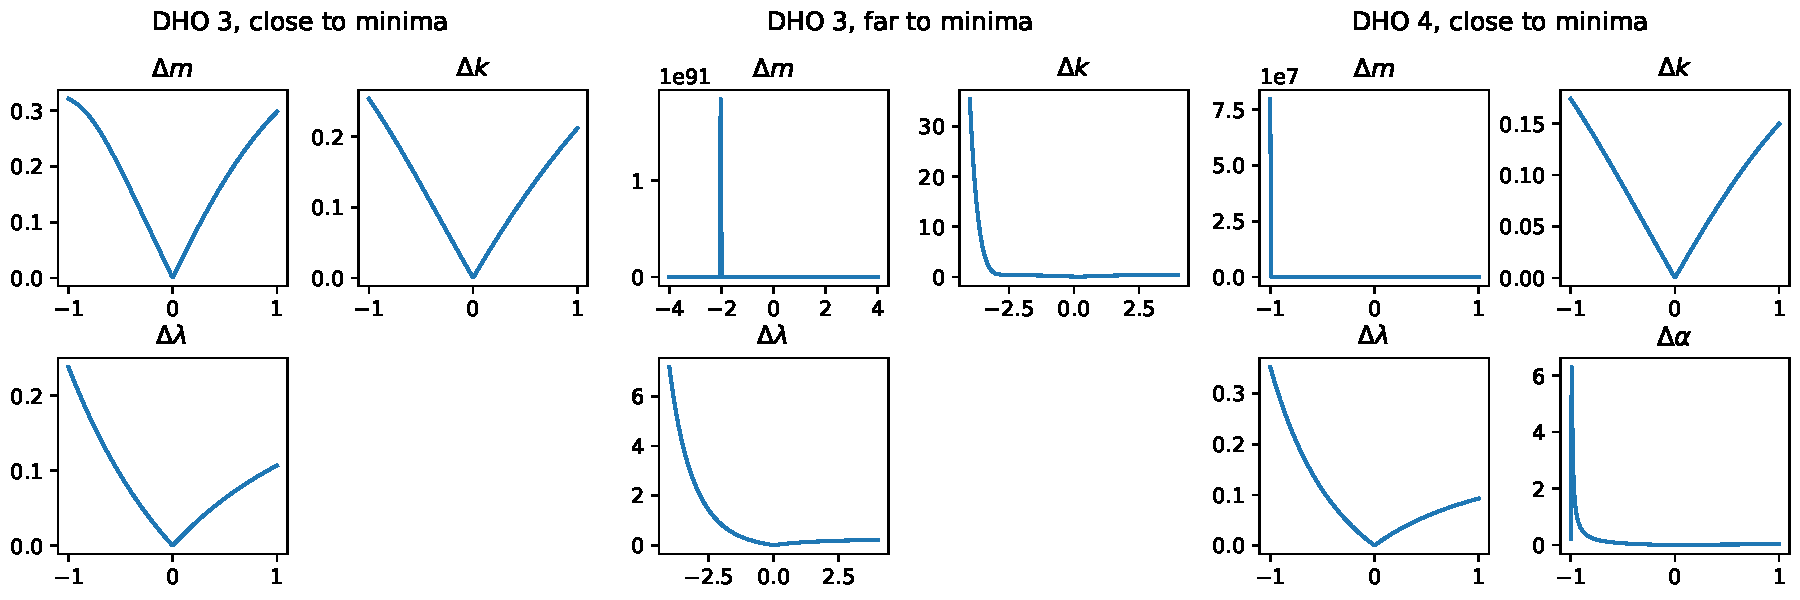
\includegraphics[width=\textwidth]{figures/loss-function-behaviour.pdf}
  \caption{The local behaviour of an equally weighted $\vbq$ and $\pi$ RMS loss function, when viewed as a function of variation in each of the embedding variables independently, with others kept fixed. We observe roughly correct behaviour in all variables bar mass $m$ and subsequently $\alpha$ for the DHO 4 embedding where $\alpha$ acts as a pre-factor for the whole non-conservative Lagrangian $\Lambda$. This behaviour is to be expected as system without mass is non-physical and explodes to infinity.}
\end{figure*}

\begin{table}
\label{table:loss-fns}
\centering
\caption{A list of loss functions. Key: RMS = Root Mean Squared, a standard loss function in machine learning%; inv-exp t.w. = inverse exponential time weighting.
}
\begin{tabular}{c|p{0.5\linewidth}}
  Name & Description \\
  \hline
  Simple RMS & Sum of RMS for $\vbq$ and $\pi$ in equal weighting. \\
  RMS-$(a, b)$ weighted & Sum of $a$ times the RMS for $\vbq$ and $b$ times the RMS for $\pi$. \\
%  RMS inv-exp t.w. & Weighting the contribution from each time-step by $e^{-t}$  \\
\end{tabular}
\end{table}

\begin{table}
\label{table:optimisation-results}
\centering
\caption{Results of optimising the chosen loss function from \tref{table:loss-fns} for $200$ initially random embeddings (distributed uniformly in $[0, 10]^n$) in the input space of the chosen embedding function, where convergence is defined as being within $\epsilon = 0.05$ of the true embedding at the end of a maximum of $250$ iterations of the optimiser. Note that for DHO 4 an additional normalisation step of dividing by $\alpha$ was applied to remove the redundancy introduced by the pre-factor in when determining if convergence had been achieved. The true embedding that was optimised towards, in DHO 3 form, was $(m = 2, k = 3, \lambda = 1)$ and systems were compared with $\Niter = 50, r = 2, \Delta t = 0.1, q_0 = 0, \pi_0 = 1$.}
\begin{tabular}{l|l|c}
  Loss function & Embedding & Convergence $\%$ \\
  \hline
  Simple RMS & DHO 3 & $33.5\%$ \\
  Simple RMS & DHO 4 & $97.5\%$ \\
  RMS-$(2, 1)$ & DHO 4 & $98\%$ \\
  RMS-$(0, 1)$ & DHO 4 & $0\%$ \\
%  RMS inv-exp t.w. & DHO 3 &
\end{tabular}
\end{table}
